\chapter{Présentation générale}

\section{Introduction}
Ce document constitue le cahier des charges du projet de \emph{système de gestion des transports} au bénéfice de la société \mo réalisé par l'assistance à maîtrise d'ouvrage \amo.

\section{\mo}

\subsection{Présentation}
Avec des dizaines de millions de volontaires dans 187 sociétés internationales, \mo est l'une des plus grandes organisations humanitaires au monde.
Elle agit avant, pendant et après les catastrophes et les urgences relatives à la santé pour répondre aux besoins des plus vulnérables et pour améliorer leur vie.
Elle dispense cette aide sans distinction de nationalité, de race, de religion, de classe ou d'opinions politiques.
\\
Elle puise sa force de son réseau de volontaires, de l'expertise basée dans la communauté et de sa capacité à donner une voix mondiale aux personnes vulnérables. Elle travaille en tant que partenaire dans le développement, la réponse aux catastrophes, l'aide pour une vie saine et sure, et l'amélioration des normes humanitaires. Le résultat : Elle aide à réduire les vulnérabilités, et rend les communautés plus résistantes.

\section{Contexte métier}
\mo possèdent des équipes de spécialistes formés aux interventions d'urgence dans le cadre notamment de catastrophes naturelles (tsunamis, tremblements de terre...).
Cinq domaines de compétence y sont représentés~:
\begin{itemize}
	\item médecine~;
	\item eau et sanitaire~;
	\item distribution~;
	\item logistique~;
	\item télécoms.
\end{itemize}
Leur dépendances respectives sont décrites dans la Figure \ref{dep}.
\begin{figure}[htbp]
	\centering
	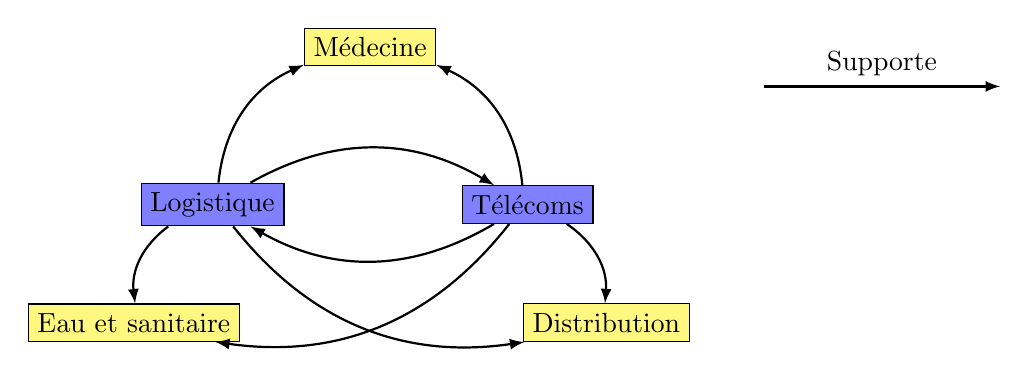
\begin{tikzpicture}
		% définition des styles
		\tikzstyle{metier}=[rectangle,draw,fill=yellow!50,text=black]
		\tikzstyle{support}=[rectangle,draw,fill=blue!50,text=black]
		\tikzstyle{supporte}=[->,>=latex,thick,rounded corners=4pt]
		% les nœuds
		\node[metier] (e) at (-3,-3) {Eau et sanitaire};
		\node[metier] (m) at (0,0.5) {Médecine};
		\node[metier] (d) at (3,-3) {Distribution};
		\node[support] (l) at (-2,-1.5) {Logistique};
		\node[support] (t) at (2,-1.5) {Télécoms};
		% les flèches
		\draw[supporte] (l) to[bend left] (t);
		\draw[supporte] (l) to[bend right] (e);
		\draw[supporte] (l) to[bend left] (m);
		\draw[supporte] (l) to[bend right] (d);
		\draw[supporte] (t) to[bend left] (l);
		\draw[supporte] (t) to[bend left] (e);
		\draw[supporte] (t) to[bend right] (m);
		\draw[supporte] (t) to[bend left] (d);
		% la légende
		\draw[supporte] (5,0) -- (8,0) node[midway,above]{Supporte};
	\end{tikzpicture}
	\caption{Dépendances entre les métiers}
	\label{dep}
\end{figure}

\subsubsection{La logistique}
L'efficacité de l'aide apportée aux populations sinistrées repose en particulier sur celle des processus logistiques.
De ce fait, la logistique apparaît comme un service support aux métiers (secteur médical, distribution, eau et sanitaires), sans lequel ils ne peuvent accomplir leurs missions.
\\
Actuellement, la logistique est confronté aux complications suivantes~:
\begin{itemize}
	\item la communication \& le partage d'informations sont peu efficaces~;
	\item les informations sont parfois redondantes~;
	\item les contraintes techniques \& environnementales~;
	\item la location de matériel donne lieu à la création de documents qui sont jusqu'à présent réalisés manuellement.
\end{itemize}

\paragraph{Processus et fonctions clefs de la logistique}
Différents processus concourent à l'accomplissement des missions logistiques dont~:
\begin{itemize}
	\item le processus d'achat~;
	\item le processus de stockage~;
	\item le processus de transport.
\end{itemize}
L'ensemble des processus doit permettre de répondre aux fonctions clefs de la logistique que sont notamment~:
\begin{itemize}
	\item planification/évaluation~;
	\item acquisition/achat~;
	\item organisation des transports~;
	\item gestion des entrepôts~;
	\item suivi et compte rendu~;
	\item standardisation~;
	\item formation et renforcement des capacités.
\end{itemize}

\paragraph{Les logisticiens de terrain}
En général, les équipes de logisticiens restent de dimension réduite (cinq à six personnes, dont un chef d'équipe), avec des profils spécialisés qui assurent en particulier des activités telles que~:
\begin{itemize}
	\item la mise en place et le maintien des procédures logistiques standards~;
	\item l'achat des biens et des services~;
	\item la facilitation de l'importation et de l'exportation des marchandises~;
	\item l'organisation du déploiement et du transport de la marchandise jusqu'aux sites de distribution~;
	\item l'organisation et la gestion des entrepôts~;
\end{itemize}
Chaque équipe reste déployée sur le terrain un mois (7j/7) et une mission d'urgence dure au plus quatre mois, délai au-delà duquel, la reconstruction prend le pas sur l'urgence.

\paragraph{Les transports}
Les transports occupent une place importante au sein de la chaîne logistique et répondent à deux grands types de services~:
\begin{itemize}
	\item le transport de personnes (les délégués)~;
	\item le transport de biens (NFI, ...).
\end{itemize}
Sauf cas exceptionnel, dans les premiers temps qui suivent une catastrophe, l'organisation ne dispose pas sur le terrain de ses propres moyens de transport de biens.
Les sociétés nationales de l'Organisation ne disposent pas en général non plus de ces moyens.
Il est alors du ressort de la logistique et en particulier du gestionnaire de flotte de trouver localement (entreprises privées, par exemple) les moyens de transport nécessaires (en général routiers).

\paragraph{Les outils}
Au cours du temps, avec l'expérience des catastrophes, l'Organisation a développé un certain nombre d'outils informatiques de terrain afin de l'aider dans ses tâches logistiques.
Parmi ces outils, figure notamment un logiciel qui permet aux équipes de disposer du suivi des biens dès lors que ceux-ci sont pris en charge au sein de la chaîne logistique sur le terrain et qui permet notamment de faciliter la traçabilité nécessaire afin de répondre aux attentes des parties prenantes, comme les donateurs notamment.

\section{Objectifs}

\subsection{Finalités}
Le but du projet est d'offrir une solution de type Transport~Management~System (appelé ci-après TMS) afin d'optimiser les ressources logistiques.
Grâce au TMS, \mo espère améliorer la qualité de ses services en se dotant d'un outil permettant de~:
\begin{itemize}
	\item \emph{planifier} les trajets, les chargements et déchargements, les dates de livraison~;
	\item \emph{réaliser} les opérations logistiques en temps voulu~;
	\item \emph{suivre} les transports et ainsi produire des documents synthétisant l'ensemble d'un trajet ou d'une cargaison~;
	\item \emph{améliorer} les processus existants grâce (entre autres) à l'établissement de statistiques permettant une mesure de l'efficience.
\end{itemize}
\mo espère ainsi, grâce à l'assistance de l'outil et l'automatisation de certaines de ces tâches, améliorer le fonctionnement global de l'organisation en suivant la logique décrite dans la Figure \ref{arbre_probleme}.

\subsection{Espérance de retour sur investissement}
\mo espère que le TMS lui permettra non seulement de réduire les coûts relatifs à la logistique mais également de maintenir son professionnalisme, améliorant ainsi son image de marque par preuve de son efficacité et de son efficience sur le terrain.
\begin{figure}[htbp] % Arbre à problèmes
	\centering
	\begin{tikzpicture} [
			node distance = 1cm, auto,font=\footnotesize,
			% STYLES
			every node/.style={node distance=3cm},
			% The comment style is used to describe the characteristics of each force
			comment/.style={rectangle, inner sep= 5pt, text width=4cm, node distance=0.25cm, font=\scriptsize\sffamily},
			% The force style is used to draw the forces' name
			force/.style={rectangle, draw, fill=black!10, inner sep=5pt, text width=4cm, text badly centered, minimum height=1.2cm, font=\bfseries\normalsize\sffamily}
		] 
		% Nodes
		\node [force] (confiance) {Confiance\\{\normalfont\footnotesize Envers \mo}};
		\node [force, above of=confiance] (transparent) {Transparence des informations\\{\normalfont\footnotesize Grâce au suivi détaillé}};
		%% Mj %% Bug avec 'X[cm] of transparent' -> Mise ne commentaire et réécriture sans
		\node [force, right=1cm of transparent] (serieux) {Sérieux\\{\normalfont\footnotesize Car on peut justifier à tout moment de l'utilisation des ressources}};
		\node [force, left=1cm of transparent] (pro) {Professionnalisme\\{\normalfont\footnotesize Notamment grâce à la planification et à l'utilisation optimale du matériel}};
		\node [force, below of=confiance, left=-1cm of confiance] (don) {Dons à l'organisation};
		\node [force, below of=confiance, right=-1cm of confiance] (benevolat) {Hausse du bénévolat};
%		\node [force, right] (serieux) {Sérieux\\{\normalfont\footnotesize Car on peut justifier à tout moment de l'utilisation des ressources}};
%		\node [force, left] (pro) {Professionnalisme\\{\normalfont\footnotesize Notamment grâce à la planification et à l'utilisation optimale du matériel}};
%		\node [force, below of=confiance, left] (don) {Dons à l'organisation};
%		\node [force, below of=confiance, right] (benevolat) {Hausse du bénévolat};
		% Draw the links between forces
		\path[->,thick]
			(don) edge (confiance)
			(benevolat) edge (confiance)
			(confiance) edge (transparent)
			(confiance) edge (serieux)
			(confiance) edge (pro);
		\end{tikzpicture} 
	\caption{Arbre à problème~: finalité du projet et retour sur investissement}
	\label{arbre_probleme}
\end{figure}

\section{Contexte de réalisation}

\subsection{Études déjà effectuées}
Une étude des scenarii possibles quant aux possibilités de l'organisation de se doter d'une solution logicielle adéquate a montré que les produits présents sur le marché ne répondaient qu'imparfaitement aux attentes de l'Organisation~:
\begin{itemize}
	\item inadéquation des solutions à certaines contraintes spécifiques du contexte d'urgence (moyens de communication à haut débit déficients...)~;
	\item solutions propriétaires~;
	\item solutions trop complexes~;
	\item solutions onéreuses.
\end{itemize}
Le scénario retenu est de fait celui d'un développement spécifique (basé éventuellement sur un noyau public) dont les fonctionnalités pourraient s'enrichir au cours du temps, avec des investissements progressifs.

\subsection{Nature des prestations demandées}
\mo cherche donc un prestataire pour la réalisation d'une solution complète de type TMS qui devra s'intégrer sans perturber le bon fonctionnement des processus existants. La solution pourra être basée sur un noyau public existant.
\\
Les prestations attendues sont~:
\begin{itemize}
	\item la suite logicielle~;
	\item le matériel (si nécessaire)~;
	\item le service support.
\end{itemize}

\subsection{Situation du projet par rapport aux autres projets de l'Organisation}
Ce projet s'intégrant à une infrastructure informatique déjà existante, cette partie tient compte des autres projets menés en parallèles et susceptibles d'impacter sur celui-ci.

\subsubsection{Migration des serveurs}
Une migration des serveurs de \mo est actuellement en projet.
Il s'agirait de migrer d'un environnement Microsoft~Windows actuellement en place, vers une distribution GNU/Linux dont le détail n'est pas encore connu.
Aucune date n'a encore été arrêtée.

\subsection{Suites prévues}
Les évolutions futures pourront être~:
\begin{itemize}
	\item ajout de fonctionnalités pour l'intégration de diverses composantes métier de \mo~;
	\item portage sur d'autres systèmes d'exploitation~;
	\item ...
\end{itemize}

\subsection{Parties concernées}

\subsubsection{Directement}
Les logisticiens de \mo en seront les principaux utilisateurs.
Le secrétariat central, par exemple, assurera le suivi de l'ensemble de la logistique à l'aide de cet outil.
Les métiers auront également accès aux informations relatives au matériel attendu ou à livrer.

\subsubsection{Indirectement}
Le temps gagné grâce à la solution permettra un acheminement plus rapide des marchandises, denrées, et personnels~; ce temps est crucial en situation d'urgence.
L'économie réalisée permettra d'augmenter les capacités, et les moyens d'action de l'association dans ses activités.
\\
Les victimes prises en charge seront donc indirectement bénéficiaires.

\subsection{Caractère confidentiel s'il y a lieu}
\mo se rapproche d'une autre association par ses activités métier et son mode de fonctionnement.
Bien que cette autre association puisse bénéficier de ce projet, il conviendra de ne pas faire de rapprochement avec celle-ci tant que sa participation au projet ne sera pas officiellement engagée.

\section{Énoncé du besoin}
Il est attendu de la solution qu'elle fonctionne sur l'architecture générale présentée dans la figure \ref{ArchitectureGenerale}.
\begin{figure}[htbp]
	\centering
	\begin{tikzpicture}
		% Définition des styles
		\tikzstyle{sup} = [rectangle,draw=white,text=black,text centered,minimum width=20mm,minimum height=80mm]
		\tikzstyle{one} = [fill=colone,rectangle,draw=white,minimum width=20mm]
		\tikzstyle{two} = [fill=coltwo,rectangle,draw=white,minimum width=20mm]
		\tikzstyle{three} = [fill=colthree,rectangle,draw=white,minimum width=20mm]
		\tikzstyle{four} = [fill=colfour,rectangle,draw=white,minimum width=20mm]
		\tikzstyle{five} = [fill=colfive,rectangle,draw=white,minimum width=20mm]
		\tikzstyle{six} = [fill=colsix,rectangle,draw=white,minimum width=20mm]
		\tikzstyle{seven} = [fill=colseven,rectangle,draw=white,minimum width=20mm]
		\tikzstyle{inf} = [rectangle,draw=white,text=black,text centered,minimum width=20mm,minimum height=10mm]
		\tikzstyle{oneonthree} = [minimum height=26mm]
		\tikzstyle{twoonthree} = [minimum height=28mm]
		\tikzstyle{threeonthree} = [minimum height=26mm]
		\tikzstyle{oneonfour} = [minimum height=20mm]
		\tikzstyle{twoonfour} = [minimum height=20mm]
		\tikzstyle{threeonfour} = [minimum height=20mm]
		\tikzstyle{fouronfour} = [minimum height=20mm]
		\tikzstyle{arrow}=[->,>=latex,thick,rounded corners=4pt]
		% Noeuds utilisateurs
		\node[inf,one] at (  0mm, 0mm) {\centering\tiny\bfseries\scshape Utilisateurs};
		\node[one,oneonthree] (Utilisateurs) at (  0mm,18mm) {};
		\node at (  0mm,9mm) {\centering\tiny\itshape Métier};
		\node at (  0mm,19mm) {\centering\includegraphics[height=16mm]{"Logistician"}};
		\node[one,twoonthree] (Logistician) at (  0mm,45mm) {};
		\node at (  0mm,36mm) {\centering\tiny\itshape Logisticien};
		\node at (  0mm,46mm) {\centering\includegraphics[height=16mm]{"Logistician"}};
		\node[one,threeonthree] (Administrateur) at (  0mm,72mm) {};
		\node at (  0mm,63mm) {\centering\tiny\itshape Administrateur};
		\node at (  0mm,73mm) {\centering\includegraphics[height=16mm]{"Logistician"}};
		% Noeuds matériels
		\node[inf,two] at ( 20mm, 0mm) {\centering\tiny\bfseries\scshape Matériels};
		\node[two,oneonthree] (Matériels) at ( 20mm,18mm) {};
		\node at ( 20mm,9mm) {\centering\tiny\itshape Portable};
		\node at ( 20mm,19mm) {\centering\includegraphics[width=16mm]{"Laptop computer"}};
		\node[two,twoonthree] (Smartphone) at ( 20mm,45mm) {};
		\node at ( 20mm,36mm) {\centering\tiny\itshape Smartphone};
		\node at ( 20mm,46mm) {\centering\includegraphics[height=16mm]{"Smartphone"}};
		\node[two,threeonthree] (Satphone) at ( 20mm,72mm) {};
		\node at ( 20mm,63mm) {\centering\tiny\itshape Téléphone satellite};
		\node at ( 20mm,73mm) {\centering\includegraphics[height=16mm]{"Smartphone"}};
		% Noeuds application
		\node[inf,three] at ( 40mm, 0mm) {\centering\tiny\bfseries\scshape Application(s)};
		\node[three,minimum width=20mm,minimum height=80mm] (Application) at ( 40mm,45mm) {\centering};
		% Noeuds synchronisation
		\node[inf,four] at ( 60mm, 0mm) {\centering\tiny\bfseries\scshape Synchro};
		\node[four,oneonfour] (Physique1) at ( 60mm,15mm) {};
		\node at ( 60mm, 9mm) {\centering\tiny\itshape Physique};
		\node at ( 56mm,16mm) {\centering\includegraphics[width=6mm]{"Compact disk"}};
		\node at ( 64mm,16mm) {\centering\includegraphics[width=8mm]{"USB key"}};
		\node[four,twoonfour] (Internet1) at ( 60mm,35mm) {};
		\node at ( 60mm,29mm) {\centering\tiny\itshape Internet};
		\node at ( 60mm,36mm) {\centering\includegraphics[width=16mm]{"Internet"}};
		\node[four,threeonfour] (Téléphonie1) at ( 60mm,55mm) {};
		\node at ( 60mm,49mm) {\centering\tiny\itshape Téléphonie};
		\node at ( 60mm,56mm) {\centering\includegraphics[height=16mm]{"Phone antenna"}};
		\node[four,fouronfour] (Satellite1) at ( 60mm,75mm) {};
		\node at ( 60mm,69mm) {\centering\tiny\itshape Satellite};
		\node at ( 60mm,76mm) {\centering\includegraphics[height=16mm]{"Satellite"}};
		% Noeuds serveur local
		\node[inf,five] at ( 80mm, 0mm) {\centering\tiny\bfseries\scshape\begin{tabular}{c}Serveur \\ local\end{tabular}};
		\node[five,minimum height=80mm] (Server1) at (80mm,45mm) {};
		\node at (80mm,34mm) {\centering\tiny\itshape Serveur};
		\node at (80mm,48mm) {\centering\includegraphics[width=16mm]{"Server"}};
		% Noeuds synchronisation
		\node[inf,six] at (100mm, 0mm) {\centering\tiny\bfseries\scshape Synchro};
		\node[six,oneonfour] (Physique1) at (100mm,15mm) {};
		\node at (100mm, 9mm) {\centering\tiny\itshape Physique};
		\node at ( 96mm,16mm) {\centering\includegraphics[width=6mm]{"Compact disk"}};
		\node at (104mm,16mm) {\centering\includegraphics[width=8mm]{"USB key"}};
		\node[six,twoonfour] (Internet2) at (100mm,35mm) {};
		\node at (100mm,29mm) {\centering\tiny\itshape Internet};
		\node at (100mm,36mm) {\centering\includegraphics[width=16mm]{"Internet"}};
		\node[six,threeonfour] (Téléphonie2) at (100mm,55mm) {};
		\node at (100mm,49mm) {\centering\tiny\itshape Téléphonie};
		\node at (100mm,56mm) {\centering\includegraphics[height=16mm]{"Phone antenna"}};
		\node[six,fouronfour] (Satellite2) at (100mm,75mm) {};
		\node at (100mm,69mm) {\centering\tiny\itshape Satellite};
		\node at (100mm,76mm) {\centering\includegraphics[height=16mm]{"Satellite"}};
		% Noeuds serveur central
		\node[inf,seven] at (120mm, 0mm) {\centering\tiny\bfseries\scshape\begin{tabular}{c}Serveur \\ central\end{tabular}};
		\node[seven,minimum height=80mm] (Server2) at (120mm,45mm) {};
		\node at (120mm,34mm) {\centering\tiny\itshape Serveur};
		\node at (120mm,48mm) {\centering\includegraphics[width=16mm]{"Server"}};
		\end{tikzpicture}
	\caption{Architecture générale}
	\label{ArchitectureGenerale}
\end{figure}

\label{liste_exhaustive_elts_contraintes}
\subsection{Utilisateurs}
De nombreux utilisateurs de différents types seront amenés à utiliser la suite logicielle.
Ces derniers seront principalement~:
\begin{itemize}
	\item le secrétariat central~;
	\item les logisticiens de terrain~;
	\item les métiers~;
	\item les administrateurs~;
\end{itemize}

\subsection{Matériels}
\mo possède déjà de nombreux matériels normalisés décris ci-dessous.
Parmi ces derniers, il est attendu que la suite logicielle soit pleinement accessible depuis ordinateurs portables, smartphones et téléphones satellite.
\mo dispose~:
\begin{itemize}
	\item de serveurs (locaux et central) actuellement sous Microsoft~Windows (une migration vers une distribution GNU/Linux étant en projet).
		Le stockage actuel des données est pris en charge par deux SGBDR que sont MySQL~Server et SQL~Oracle~;
	\item d'ordinateurs portables sous Microsoft~Windows~7.
		Ils sont équipés de 16 Go de mémoire vive et de 250 Go d'espace disque.
		\href{https://www.microsoft.com/fr-fr/download/internet-explorer.aspx}{Microsoft~Internet~Explorer~11} et \href{http://www.mozilla.org/en-US/firefox/27.0.1/releasenotes/}{Mozilla~Firefox~27.0.1} sont les deux navigateurs présents par défaut et leur utilisation est fonction des préférences de l'utilisateur~;
	\item de terminaux satellitaires \href{http://explorersatellite.com/BGAN/thrane_thrane_bgan.html}{BGAN (Thrane \& Thrane~Explorer~500)}~;
	\item de smartphones sous \href{http://www.android.com/}{Android}~;
	\item de téléphones satellitaires Thuraya (\href{http://www.thuraya.com.kw/hughes7101.html}{Hughes~7100} / \href{http://www.thuraya.com.kw/hughes7100.html}{7101} et \href{http://www.thuraya.com.kw/so-2510.html}{SO~2510}) et Iridium (\href{http://www.iridium.com/products/Iridium-9505A-Satellite-Phone.aspx}{9505A} et \href{http://www.iridium.com/products/Iridium9555SatellitePhone.aspx}{9555}) destinés principalement à la communication vocale~;
	\item de téléphones télécopieurs (fax) satellitaires (Nera~Mini-M~Worldphone)~;
	\item de communicateurs radio VHF (Motorola~GP360/GM360)~;
	\item de points d'accès sans fil (Linksys~WRT54G) permettant de partager une connexion à large bande (BGAN, ADSL, VSAT, etc.) dans un réseau sans fil~;
	\item de GPS portables (eTrex~Venture~HC de Garmin).
\end{itemize}
\begin{constraint}[Contrainte de compatibilité]
	La suite logicielle doit impérativement être compatible avec les matériels énoncés.
	En outre, elle doit également être compatible avec les systèmes d'exploitation et, au minimum, les versions de logiciels précisés (un support pour versions ultérieurs pouvant être sollicité).
\end{constraint}
\begin{constraint}[Contrainte de coûts de communication]
	Bien que l'Organisation dispose de nombreux moyens de communications satellitaires, ces derniers sont principalement destinés aux urgences, car extrêmement coûteux.
	Un besoin fondamental est donc de minimiser ce genre de transferts, ainsi que d'avertir un utilisateur sur le point d'y avoir recours, afin de prévenir les cas d'erreur ou d'inattention.
	La priorité sur les moyens de communication utilisés devraient se plier aux préférences suivantes (par ordre décroissant)~:
	\begin{enumerate}
		\item les réseaux Internet~;
		\item les réseaux GSM~;
		\item les transports physiques~;
		\item les réseaux satellitaires.
	\end{enumerate}
\end{constraint}

\subsection{Application}
Le TMS doit~:
\begin{itemize}
	\item permettre une planification \& un suivi des transports~;
	\item être multilingue~;
	\item avoir des interfaces utilisateurs personnalisées dépendant de la fonction de l'utilisateur~;
	\item mémoriser les préférences utilisateur (e.g. la langue de l'application)~;
	\item gérer explicitement la sécurité des communications~;
	\item authentifier les utilisateurs (si le contexte d'utilisation le permet)~;
	\item gérer les sauvegardes et être compatible avec les grandes solutions du marché~;
	\item gérer explicitement la synchronisation, les importations, et les exportations de données autant entre les clients et le serveur local qu'entre le serveur local et le serveur central (dans les cas où les moyens de communications sont réduits)~;
	\item produire des documents de synthèse (i.e. tableaux de bord) dont le contenu est personnalisable en fonction du destinataire~;
	\item gérer les documents internes (réquisitions, waybills/delivery notes, ...)~;
	\item gérer les documents externes (contrats, patentes, ...)~;
	\item produire des statistiques personnalisables.
\end{itemize}
